% Options for packages loaded elsewhere
\PassOptionsToPackage{unicode}{hyperref}
\PassOptionsToPackage{hyphens}{url}
%
\documentclass[
]{book}
\usepackage{amsmath,amssymb}
\usepackage{lmodern}
\usepackage{iftex}
\ifPDFTeX
  \usepackage[T1]{fontenc}
  \usepackage[utf8]{inputenc}
  \usepackage{textcomp} % provide euro and other symbols
\else % if luatex or xetex
  \usepackage{unicode-math}
  \defaultfontfeatures{Scale=MatchLowercase}
  \defaultfontfeatures[\rmfamily]{Ligatures=TeX,Scale=1}
\fi
% Use upquote if available, for straight quotes in verbatim environments
\IfFileExists{upquote.sty}{\usepackage{upquote}}{}
\IfFileExists{microtype.sty}{% use microtype if available
  \usepackage[]{microtype}
  \UseMicrotypeSet[protrusion]{basicmath} % disable protrusion for tt fonts
}{}
\makeatletter
\@ifundefined{KOMAClassName}{% if non-KOMA class
  \IfFileExists{parskip.sty}{%
    \usepackage{parskip}
  }{% else
    \setlength{\parindent}{0pt}
    \setlength{\parskip}{6pt plus 2pt minus 1pt}}
}{% if KOMA class
  \KOMAoptions{parskip=half}}
\makeatother
\usepackage{xcolor}
\usepackage{color}
\usepackage{fancyvrb}
\newcommand{\VerbBar}{|}
\newcommand{\VERB}{\Verb[commandchars=\\\{\}]}
\DefineVerbatimEnvironment{Highlighting}{Verbatim}{commandchars=\\\{\}}
% Add ',fontsize=\small' for more characters per line
\usepackage{framed}
\definecolor{shadecolor}{RGB}{248,248,248}
\newenvironment{Shaded}{\begin{snugshade}}{\end{snugshade}}
\newcommand{\AlertTok}[1]{\textcolor[rgb]{0.94,0.16,0.16}{#1}}
\newcommand{\AnnotationTok}[1]{\textcolor[rgb]{0.56,0.35,0.01}{\textbf{\textit{#1}}}}
\newcommand{\AttributeTok}[1]{\textcolor[rgb]{0.77,0.63,0.00}{#1}}
\newcommand{\BaseNTok}[1]{\textcolor[rgb]{0.00,0.00,0.81}{#1}}
\newcommand{\BuiltInTok}[1]{#1}
\newcommand{\CharTok}[1]{\textcolor[rgb]{0.31,0.60,0.02}{#1}}
\newcommand{\CommentTok}[1]{\textcolor[rgb]{0.56,0.35,0.01}{\textit{#1}}}
\newcommand{\CommentVarTok}[1]{\textcolor[rgb]{0.56,0.35,0.01}{\textbf{\textit{#1}}}}
\newcommand{\ConstantTok}[1]{\textcolor[rgb]{0.00,0.00,0.00}{#1}}
\newcommand{\ControlFlowTok}[1]{\textcolor[rgb]{0.13,0.29,0.53}{\textbf{#1}}}
\newcommand{\DataTypeTok}[1]{\textcolor[rgb]{0.13,0.29,0.53}{#1}}
\newcommand{\DecValTok}[1]{\textcolor[rgb]{0.00,0.00,0.81}{#1}}
\newcommand{\DocumentationTok}[1]{\textcolor[rgb]{0.56,0.35,0.01}{\textbf{\textit{#1}}}}
\newcommand{\ErrorTok}[1]{\textcolor[rgb]{0.64,0.00,0.00}{\textbf{#1}}}
\newcommand{\ExtensionTok}[1]{#1}
\newcommand{\FloatTok}[1]{\textcolor[rgb]{0.00,0.00,0.81}{#1}}
\newcommand{\FunctionTok}[1]{\textcolor[rgb]{0.00,0.00,0.00}{#1}}
\newcommand{\ImportTok}[1]{#1}
\newcommand{\InformationTok}[1]{\textcolor[rgb]{0.56,0.35,0.01}{\textbf{\textit{#1}}}}
\newcommand{\KeywordTok}[1]{\textcolor[rgb]{0.13,0.29,0.53}{\textbf{#1}}}
\newcommand{\NormalTok}[1]{#1}
\newcommand{\OperatorTok}[1]{\textcolor[rgb]{0.81,0.36,0.00}{\textbf{#1}}}
\newcommand{\OtherTok}[1]{\textcolor[rgb]{0.56,0.35,0.01}{#1}}
\newcommand{\PreprocessorTok}[1]{\textcolor[rgb]{0.56,0.35,0.01}{\textit{#1}}}
\newcommand{\RegionMarkerTok}[1]{#1}
\newcommand{\SpecialCharTok}[1]{\textcolor[rgb]{0.00,0.00,0.00}{#1}}
\newcommand{\SpecialStringTok}[1]{\textcolor[rgb]{0.31,0.60,0.02}{#1}}
\newcommand{\StringTok}[1]{\textcolor[rgb]{0.31,0.60,0.02}{#1}}
\newcommand{\VariableTok}[1]{\textcolor[rgb]{0.00,0.00,0.00}{#1}}
\newcommand{\VerbatimStringTok}[1]{\textcolor[rgb]{0.31,0.60,0.02}{#1}}
\newcommand{\WarningTok}[1]{\textcolor[rgb]{0.56,0.35,0.01}{\textbf{\textit{#1}}}}
\usepackage{longtable,booktabs,array}
\usepackage{calc} % for calculating minipage widths
% Correct order of tables after \paragraph or \subparagraph
\usepackage{etoolbox}
\makeatletter
\patchcmd\longtable{\par}{\if@noskipsec\mbox{}\fi\par}{}{}
\makeatother
% Allow footnotes in longtable head/foot
\IfFileExists{footnotehyper.sty}{\usepackage{footnotehyper}}{\usepackage{footnote}}
\makesavenoteenv{longtable}
\usepackage{graphicx}
\makeatletter
\def\maxwidth{\ifdim\Gin@nat@width>\linewidth\linewidth\else\Gin@nat@width\fi}
\def\maxheight{\ifdim\Gin@nat@height>\textheight\textheight\else\Gin@nat@height\fi}
\makeatother
% Scale images if necessary, so that they will not overflow the page
% margins by default, and it is still possible to overwrite the defaults
% using explicit options in \includegraphics[width, height, ...]{}
\setkeys{Gin}{width=\maxwidth,height=\maxheight,keepaspectratio}
% Set default figure placement to htbp
\makeatletter
\def\fps@figure{htbp}
\makeatother
\setlength{\emergencystretch}{3em} % prevent overfull lines
\providecommand{\tightlist}{%
  \setlength{\itemsep}{0pt}\setlength{\parskip}{0pt}}
\setcounter{secnumdepth}{5}
\usepackage{booktabs}
\usepackage{amsthm}
\makeatletter
\def\thm@space@setup{%
  \thm@preskip=8pt plus 2pt minus 4pt
  \thm@postskip=\thm@preskip
}
\makeatother
\ifLuaTeX
  \usepackage{selnolig}  % disable illegal ligatures
\fi
\usepackage[]{natbib}
\bibliographystyle{apalike}
\IfFileExists{bookmark.sty}{\usepackage{bookmark}}{\usepackage{hyperref}}
\IfFileExists{xurl.sty}{\usepackage{xurl}}{} % add URL line breaks if available
\urlstyle{same} % disable monospaced font for URLs
\hypersetup{
  pdftitle={Bookdown - Grupo B},
  pdfauthor={Andrés Peralta Alean, David Barrera Barrera, Luis Gonzalo Guerra J},
  hidelinks,
  pdfcreator={LaTeX via pandoc}}

\title{Bookdown - Grupo B}
\author{Andrés Peralta Alean, David Barrera Barrera, Luis Gonzalo Guerra J}
\date{2023-05-08}

\begin{document}
\maketitle

{
\setcounter{tocdepth}{1}
\tableofcontents
}
\hypertarget{propuesta}{%
\chapter{Propuesta}\label{propuesta}}

Análisis de riesgo crediticio y su importancia La evaluación del riesgo crediticio es una tarea crítica para cualquier empresa que ofrezca préstamos o créditos.
El incumplimiento de los términos del préstamo o la falta de pago pueden generar grandes pérdidas financieras y afectar la estabilidad de la empresa.
Es por ello que es importante contar con herramientas y técnicas que permitan evaluar el riesgo crediticio de manera eficiente.

El análisis de riesgo crediticio utiliza históricos para evaluar el comportamiento de los clientes a lo largo de varios periodos.
De esta forma, se pueden obtener patrones y características que permiten segregar grupos de clientes y determinar un posible perfil de riesgo.
Los resultados obtenidos a partir de este análisis pueden ayudar a la empresa a tomar decisiones más informadas y a reducir el riesgo crediticio.

Además, el análisis de riesgo crediticio permite identificar posibles oportunidades para la empresa.
Por ejemplo, puede ayudar a la empresa a identificar clientes que presenten un bajo riesgo crediticio y, por lo tanto, puedan recibir préstamos con tasas de interés más bajas.
De esta manera, la empresa puede aumentar su base de clientes y mejorar su rentabilidad.

En cuanto a las fuentes de información, se pueden utilizar diversas fuentes para recopilar los datos necesarios para el análisis de riesgo crediticio.
Entre ellas se encuentran bases de datos públicas y privadas, encuestas, registros gubernamentales, entre otras.
Es importante verificar la calidad de la información obtenida para asegurar la precisión y confiabilidad de los resultados.

En el caso específico de la empresa ABC, se cuenta con los permisos necesarios por parte del área de gestión de cobranzas y se eliminaron los datos personales de los clientes con los cuales se extrajeron las características.

En resumen, el análisis de riesgo crediticio es una técnica muy útil para evaluar el riesgo crediticio de los clientes y para identificar posibles oportunidades para la empresa.
Se pueden utilizar diversas fuentes de información para recopilar los datos necesarios para este análisis, pero es importante asegurarse de contar con los permisos necesarios y verificar la calidad de la información obtenida.

\hypertarget{Analisis}{%
\chapter{Analisis Exploratorio}\label{Analisis}}

\hypertarget{creacion-del-objeto-de-analisis-temporal-indice.ts}{%
\section{Creacion del objeto de analisis temporal indice.ts}\label{creacion-del-objeto-de-analisis-temporal-indice.ts}}

\hypertarget{carga-de-librerias-y-datasource}{%
\subsection{Carga de librerias y datasource}\label{carga-de-librerias-y-datasource}}

\begin{verbatim}
## Registered S3 method overwritten by 'quantmod':
##   method            from
##   as.zoo.data.frame zoo
\end{verbatim}

\begin{verbatim}
## Loading required package: zoo
\end{verbatim}

\begin{verbatim}
## 
## Attaching package: 'zoo'
\end{verbatim}

\begin{verbatim}
## The following objects are masked from 'package:base':
## 
##     as.Date, as.Date.numeric
\end{verbatim}

\begin{verbatim}
## Successfully loaded changepoint package version 2.2.4
##  See NEWS for details of changes.
\end{verbatim}

\begin{verbatim}
## # A tibble: 643,570 x 8
##    Periodo Sub_Tipo N_Clientes DIAS_DE_MORA     Saldo Genero grupo_actividad_eco
##    <chr>   <chr>         <dbl>        <dbl>     <dbl> <chr>  <chr>              
##  1 2018-01 CDC               4            0 15824105. Femen~ Dependiente privado
##  2 2018-01 CDC               1            0  6810373. Femen~ Dependiente privado
##  3 2018-01 CDC               6            6 28819502. Femen~ Dependiente privado
##  4 2018-01 CDC              12           63 81343674. Femen~ Dependiente privado
##  5 2018-01 CDC               1           21  7524344. Femen~ Dependiente privado
##  6 2018-01 CDC               4            0 12974213. Femen~ Dependiente privado
##  7 2018-01 CDC               3            1 21348609. Femen~ Dependiente privado
##  8 2018-01 CDC               2            0 11475858. Femen~ Dependiente privado
##  9 2018-01 CDC              10           38 60012355. Femen~ Dependiente privado
## 10 2018-01 CDC               1            0  9034715. Femen~ Dependiente privado
## # i 643,560 more rows
## # i 1 more variable: Cuidad_res <chr>
\end{verbatim}

\hypertarget{modificamos-el-df-para-que-tenga-el-formato-adecuado-y-lo-mostramos}{%
\subsection{Modificamos el df para que tenga el formato adecuado y lo mostramos}\label{modificamos-el-df-para-que-tenga-el-formato-adecuado-y-lo-mostramos}}

\begin{Shaded}
\begin{Highlighting}[]
\CommentTok{\# Cambio el tipo de dato de la columna temporal(Periodo)}
\NormalTok{datos}\SpecialCharTok{$}\NormalTok{Periodo }\OtherTok{\textless{}{-}} \FunctionTok{as.Date}\NormalTok{(}\FunctionTok{paste0}\NormalTok{(datos}\SpecialCharTok{$}\NormalTok{Periodo, }\StringTok{"{-}01"}\NormalTok{))}

\CommentTok{\# Consolido el df en funcion de la variable de interes (Saldo)}
\NormalTok{datos }\OtherTok{\textless{}{-}} \FunctionTok{aggregate}\NormalTok{(Saldo }\SpecialCharTok{\textasciitilde{}}\NormalTok{ Periodo, }\AttributeTok{data =}\NormalTok{ datos, sum)}

\CommentTok{\# Genero mi objeto ts para el analisis}
\NormalTok{indice.ts }\OtherTok{\textless{}{-}} \FunctionTok{ts}\NormalTok{(datos}\SpecialCharTok{$}\NormalTok{Saldo, }\AttributeTok{start =} \FunctionTok{c}\NormalTok{(}\DecValTok{2018}\NormalTok{,}\DecValTok{1}\NormalTok{), }\AttributeTok{frequency =} \DecValTok{12}\NormalTok{)}
\NormalTok{indice.ts}
\end{Highlighting}
\end{Shaded}

\begin{verbatim}
##               Jan          Feb          Mar          Apr          May
## 2018 2.562223e+12 2.601532e+12 2.653315e+12 2.717915e+12 2.852608e+12
## 2019 3.732137e+12 3.810740e+12 3.923380e+12 3.995810e+12 4.092819e+12
## 2020 2.022405e+12 4.295886e+12 4.304185e+12 4.195404e+12 4.177219e+12
## 2021 4.369300e+12 4.478002e+12 4.595047e+12 4.627874e+12 4.705783e+12
## 2022 6.351501e+12 6.555819e+12 6.739823e+12 6.925001e+12 7.132542e+12
## 2023 8.083445e+12 7.951094e+12 7.812947e+12 7.765132e+12             
##               Jun          Jul          Aug          Sep          Oct
## 2018 2.986446e+12 3.102493e+12 3.196138e+12 3.272388e+12 3.394038e+12
## 2019 4.164386e+12 4.198177e+12 4.267921e+12 4.307340e+12 4.113506e+12
## 2020 4.164434e+12 4.082507e+12 4.067948e+12 4.120926e+12 4.182877e+12
## 2021 4.846473e+12 4.983882e+12 5.091594e+12 5.385784e+12 5.730839e+12
## 2022 7.435792e+12 7.529328e+12 7.670212e+12 7.789046e+12 7.903472e+12
## 2023                                                                 
##               Nov          Dec
## 2018 3.617129e+12 3.690229e+12
## 2019 4.314034e+12 4.455499e+12
## 2020 4.344709e+12 4.384188e+12
## 2021 5.955740e+12 6.164705e+12
## 2022 8.115444e+12 8.154174e+12
## 2023
\end{verbatim}

\hypertarget{graficamos-la-serie}{%
\subsection{Graficamos la serie}\label{graficamos-la-serie}}

\begin{Shaded}
\begin{Highlighting}[]
\FunctionTok{plot}\NormalTok{(indice.ts, }\AttributeTok{main =} \StringTok{""}\NormalTok{,}\AttributeTok{ylab=}\StringTok{"valor"}\NormalTok{,}\AttributeTok{col=}\StringTok{"deepskyblue"}\NormalTok{,}\AttributeTok{xlab=}\StringTok{"Periodos"}\NormalTok{)}
\FunctionTok{title}\NormalTok{(}\AttributeTok{main =} \StringTok{"Saldos Mensuales Clientes"}\NormalTok{)}
\end{Highlighting}
\end{Shaded}

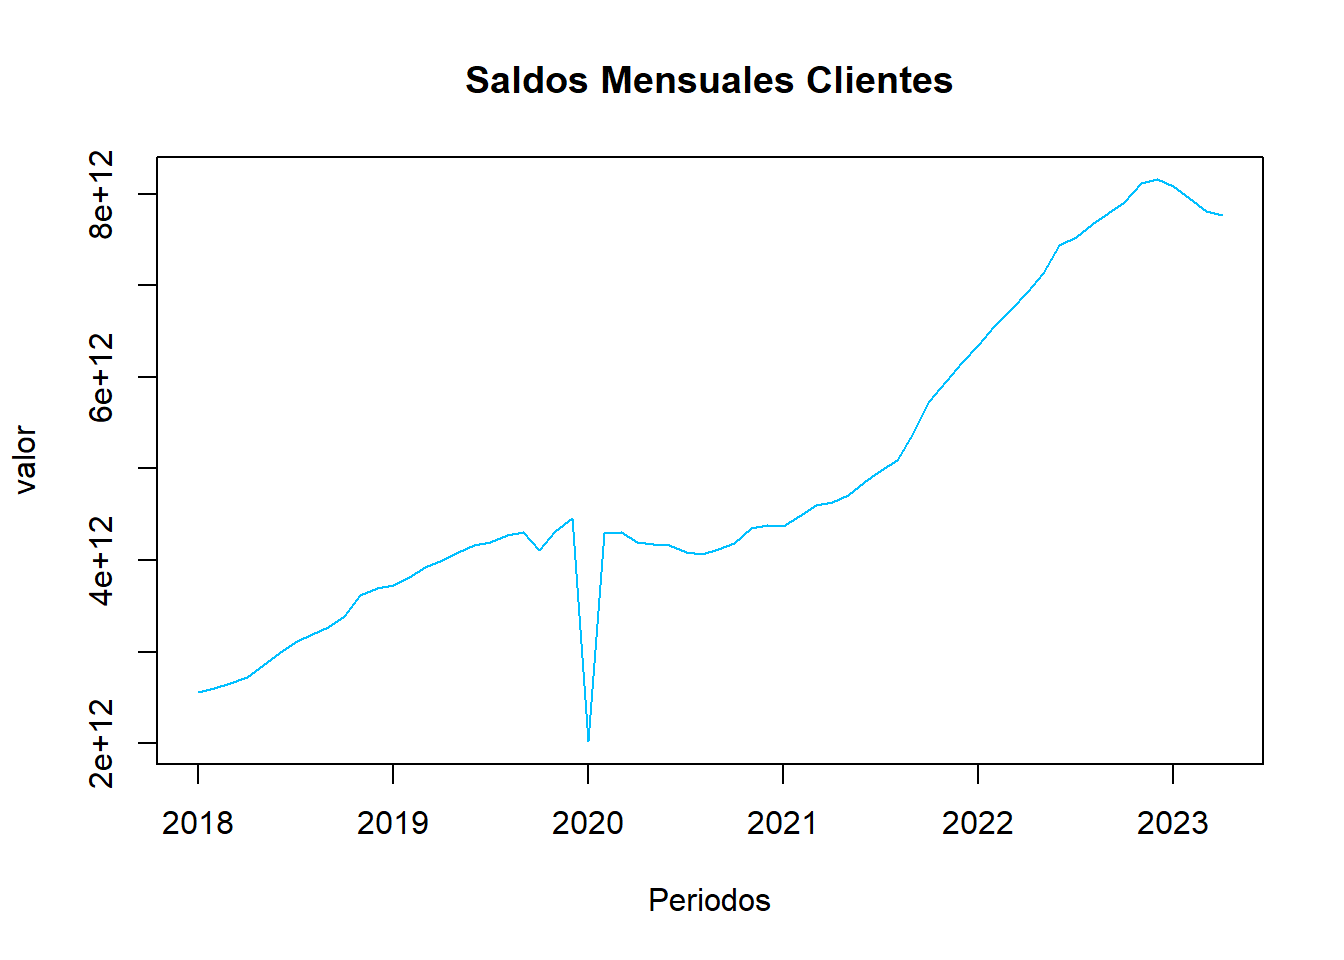
\includegraphics{bookdown-demo_files/figure-latex/unnamed-chunk-3-1.pdf}

\hypertarget{chequeos-basicos-para-confirmar-la-estructura-del-contenedor-ts}{%
\subsection{Chequeos basicos para confirmar la estructura del contenedor ts}\label{chequeos-basicos-para-confirmar-la-estructura-del-contenedor-ts}}

\begin{verbatim}
## [1] "El tipo de datos del df indice.ts es: "
\end{verbatim}

\begin{verbatim}
## [1] "ts"
\end{verbatim}

\begin{verbatim}
## [1] "La serie de tiempo indice.ts empieza en: "
\end{verbatim}

\begin{verbatim}
## [1] 2018    1
\end{verbatim}

\begin{verbatim}
## [1] "La serie de tiempo indice.ts termina en: "
\end{verbatim}

\begin{verbatim}
## [1] 2023    4
\end{verbatim}

\hypertarget{analisis-descriptivo}{%
\section{Analisis Descriptivo}\label{analisis-descriptivo}}

\hypertarget{grafica-de-rezagos}{%
\subsection{Grafica de Rezagos}\label{grafica-de-rezagos}}

\begin{Shaded}
\begin{Highlighting}[]
\FunctionTok{lag.plot}\NormalTok{(indice.ts, }\DecValTok{9}\NormalTok{ , }\AttributeTok{do.lines =} \ConstantTok{FALSE}\NormalTok{)}
\end{Highlighting}
\end{Shaded}

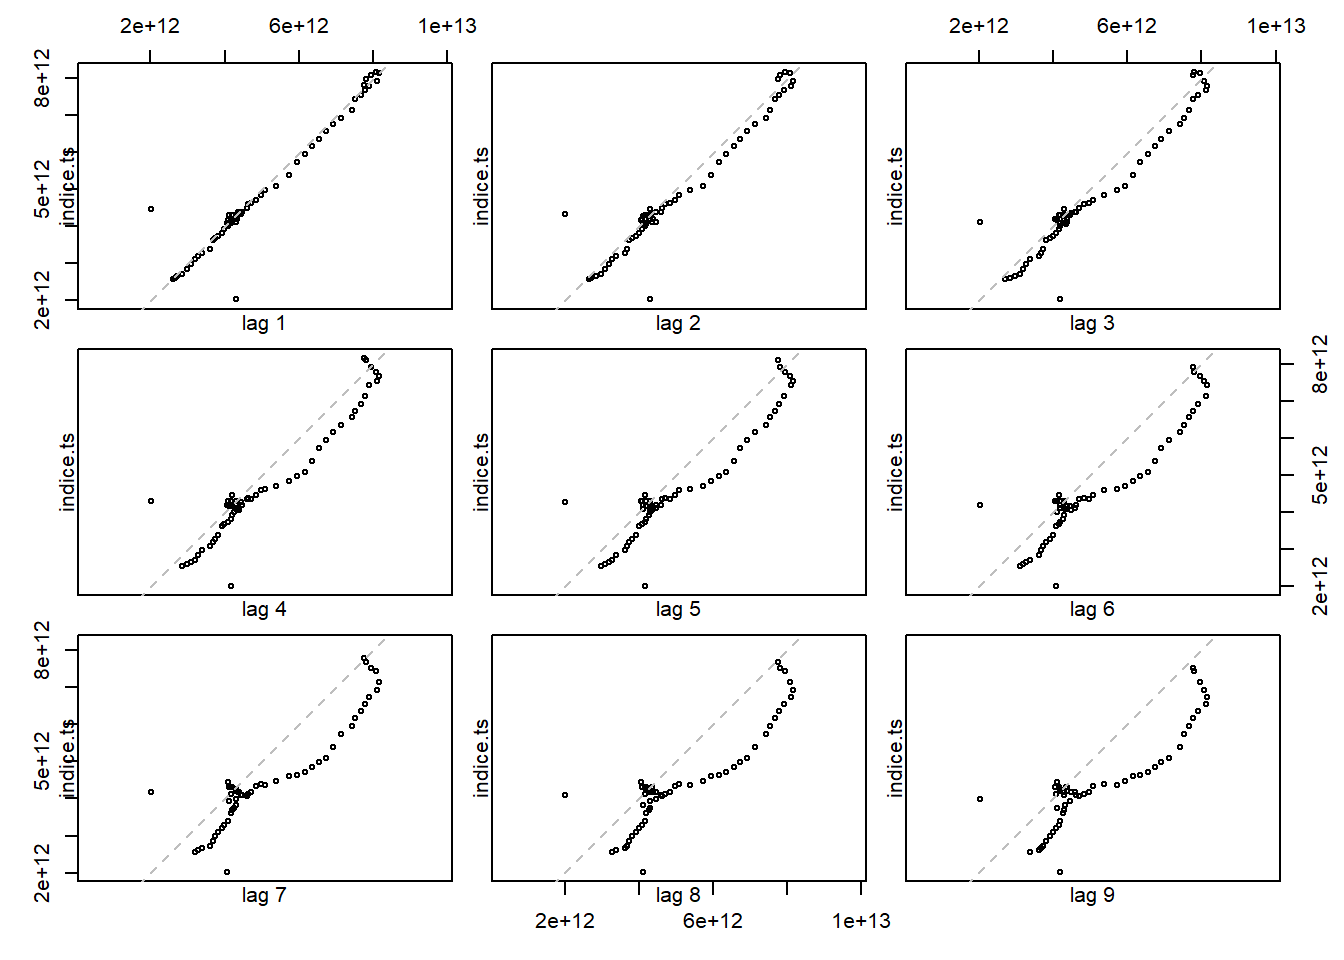
\includegraphics{bookdown-demo_files/figure-latex/unnamed-chunk-5-1.pdf}
Conclusion: Se observa con claridad que existe una tendencia XXXXXX

\hypertarget{media-movil}{%
\subsection{Media Movil}\label{media-movil}}

Crearemos a continuacion 3 medias moviles para el objeto ts. Estas tendran 3, 5 y 7 periodos para su calculo.

\begin{Shaded}
\begin{Highlighting}[]
\NormalTok{mm3 }\OtherTok{\textless{}{-}} \FunctionTok{rollmean}\NormalTok{(indice.ts,}\AttributeTok{k=}\DecValTok{3}\NormalTok{)}
\FunctionTok{cat}\NormalTok{(}\StringTok{"Media Movil con 3 meses: "}\NormalTok{, mm3,}\StringTok{"}\SpecialCharTok{\textbackslash{}n\textbackslash{}n}\StringTok{"}\NormalTok{)}
\end{Highlighting}
\end{Shaded}

\begin{verbatim}
## Media Movil con 3 meses:  2.60569e+12 2.657587e+12 2.741279e+12 2.852323e+12 2.980516e+12 3.095026e+12 3.19034e+12 3.287521e+12 3.427851e+12 3.567132e+12 3.679831e+12 3.744369e+12 3.822086e+12 3.909977e+12 4.004003e+12 4.084338e+12 4.151794e+12 4.210161e+12 4.257812e+12 4.229589e+12 4.24496e+12 4.294346e+12 3.597313e+12 3.591264e+12 3.540826e+12 4.265159e+12 4.225603e+12 4.179019e+12 4.141387e+12 4.104963e+12 4.090461e+12 4.123917e+12 4.216171e+12 4.303925e+12 4.366066e+12 4.410497e+12 4.480783e+12 4.566974e+12 4.642901e+12 4.72671e+12 4.845379e+12 4.973983e+12 5.153753e+12 5.402739e+12 5.690788e+12 5.950428e+12 6.157316e+12 6.357342e+12 6.549048e+12 6.740214e+12 6.932456e+12 7.164445e+12 7.365887e+12 7.545111e+12 7.662862e+12 7.787577e+12 7.935987e+12 8.057696e+12 8.117688e+12 8.062904e+12 7.949162e+12 7.843058e+12
\end{verbatim}

\begin{Shaded}
\begin{Highlighting}[]
\NormalTok{mm5 }\OtherTok{\textless{}{-}} \FunctionTok{rollmean}\NormalTok{(indice.ts,}\AttributeTok{k=}\DecValTok{5}\NormalTok{)}
\FunctionTok{cat}\NormalTok{(}\StringTok{"Media Movil con 5 meses: "}\NormalTok{, mm5,}\StringTok{"}\SpecialCharTok{\textbackslash{}n\textbackslash{}n}\StringTok{"}\NormalTok{)}
\end{Highlighting}
\end{Shaded}

\begin{verbatim}
## Media Movil con 5 meses:  2.677519e+12 2.762363e+12 2.862556e+12 2.97112e+12 3.082015e+12 3.190301e+12 3.316437e+12 3.433984e+12 3.541184e+12 3.648854e+12 3.754723e+12 3.830459e+12 3.910977e+12 3.997427e+12 4.074914e+12 4.143823e+12 4.206128e+12 4.210266e+12 4.240195e+12 4.29166e+12 3.842557e+12 3.840266e+12 3.878402e+12 3.854676e+12 3.79902e+12 4.227426e+12 4.18475e+12 4.137503e+12 4.122607e+12 4.123739e+12 4.159794e+12 4.22013e+12 4.2804e+12 4.351815e+12 4.434249e+12 4.490882e+12 4.555201e+12 4.650636e+12 4.751812e+12 4.851121e+12 5.002703e+12 5.207714e+12 5.429568e+12 5.665732e+12 5.917714e+12 6.151721e+12 6.353518e+12 6.54737e+12 6.740937e+12 6.957795e+12 7.152497e+12 7.338575e+12 7.511384e+12 7.66557e+12 7.8015e+12 7.92647e+12 8.009116e+12 8.041526e+12 8.023421e+12 7.953359e+12
\end{verbatim}

\begin{Shaded}
\begin{Highlighting}[]
\NormalTok{mm7 }\OtherTok{\textless{}{-}} \FunctionTok{rollmean}\NormalTok{(indice.ts,}\AttributeTok{k=}\DecValTok{7}\NormalTok{)}
\FunctionTok{cat}\NormalTok{(}\StringTok{"Media Movil con 7 meses: "}\NormalTok{, mm7)}
\end{Highlighting}
\end{Shaded}

\begin{verbatim}
## Media Movil con 7 meses:  2.782362e+12 2.872921e+12 2.968758e+12 3.074575e+12 3.203034e+12 3.322694e+12 3.429222e+12 3.5304e+12 3.634291e+12 3.737637e+12 3.837463e+12 3.915643e+12 3.988207e+12 4.064748e+12 4.13569e+12 4.162851e+12 4.208312e+12 4.260123e+12 3.954126e+12 3.968084e+12 3.973265e+12 3.957274e+12 3.966376e+12 3.945005e+12 3.89172e+12 4.183941e+12 4.158946e+12 4.141617e+12 4.162946e+12 4.192513e+12 4.221779e+12 4.278279e+12 4.353579e+12 4.426e+12 4.5007e+12 4.572381e+12 4.658052e+12 4.761236e+12 4.89092e+12 5.053176e+12 5.242871e+12 5.451288e+12 5.666292e+12 5.890855e+12 6.126316e+12 6.346204e+12 6.546447e+12 6.757883e+12 6.952829e+12 7.141217e+12 7.317392e+12 7.483628e+12 7.653691e+12 7.799638e+12 7.89216e+12 7.952412e+12 7.972803e+12 7.969387e+12
\end{verbatim}

Veamos como es el comportamiento de las mismas en comparacion con lod datos originales de la serie de tiempo

\begin{Shaded}
\begin{Highlighting}[]
\FunctionTok{plot}\NormalTok{(}\DecValTok{1}\SpecialCharTok{:}\FunctionTok{length}\NormalTok{(indice.ts), indice.ts, }\AttributeTok{type =} \StringTok{"l"}\NormalTok{,   }
     \AttributeTok{ylim =} \FunctionTok{c}\NormalTok{(}\FunctionTok{min}\NormalTok{(indice.ts), }\FunctionTok{max}\NormalTok{(indice.ts)),}
     \AttributeTok{xlab =} \StringTok{"Lineas de Serie de Tiempo"}\NormalTok{, }\AttributeTok{ylab =} \StringTok{"Valores"}\NormalTok{)}
\FunctionTok{lines}\NormalTok{(}\DecValTok{1}\SpecialCharTok{:}\FunctionTok{length}\NormalTok{(mm3),mm3,}\AttributeTok{type =} \StringTok{"l"}\NormalTok{, }\AttributeTok{col=}\DecValTok{2}\NormalTok{)}
\FunctionTok{lines}\NormalTok{(}\DecValTok{1}\SpecialCharTok{:}\FunctionTok{length}\NormalTok{(mm5),mm5,}\AttributeTok{type =} \StringTok{"l"}\NormalTok{, }\AttributeTok{col=}\DecValTok{3}\NormalTok{)}
\FunctionTok{lines}\NormalTok{(}\DecValTok{1}\SpecialCharTok{:}\FunctionTok{length}\NormalTok{(mm7),mm7,}\AttributeTok{type =} \StringTok{"l"}\NormalTok{, }\AttributeTok{col=}\DecValTok{4}\NormalTok{)}
\FunctionTok{legend}\NormalTok{(}\StringTok{"topleft"}\NormalTok{,}
       \FunctionTok{c}\NormalTok{(}\StringTok{"Indice.Ts"}\NormalTok{, }\StringTok{"Media Movil 3 Meses"}\NormalTok{, }\StringTok{"Media Movil 5 Meses"}\NormalTok{, }\StringTok{"Media Movil 7 Meses"}\NormalTok{),}
       \AttributeTok{lty =} \DecValTok{1}\NormalTok{, }\AttributeTok{col =} \DecValTok{1}\SpecialCharTok{:}\DecValTok{4}\NormalTok{)}
\end{Highlighting}
\end{Shaded}

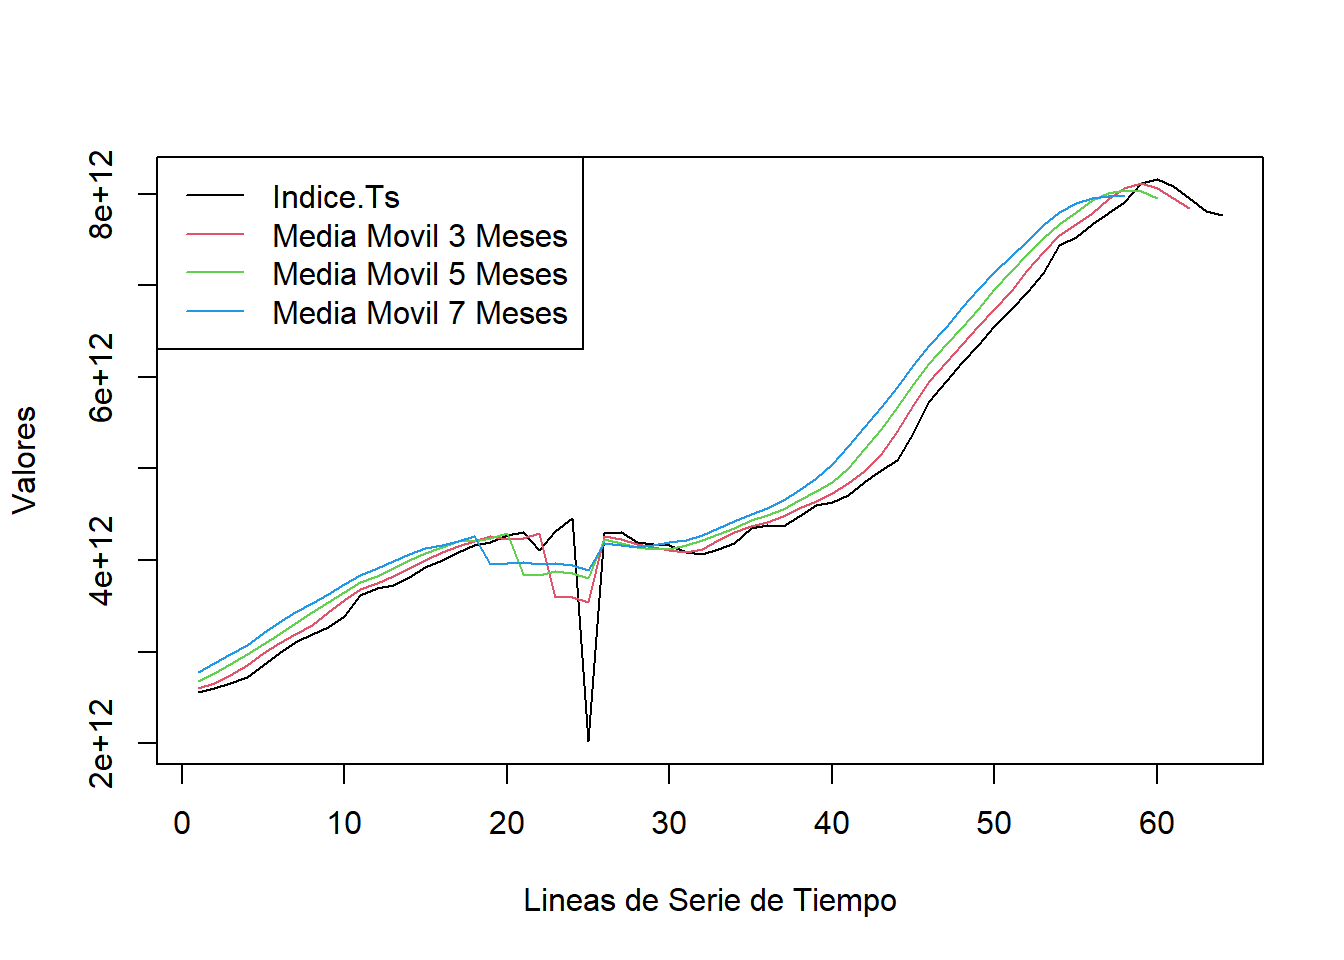
\includegraphics{bookdown-demo_files/figure-latex/unnamed-chunk-7-1.pdf}

\hypertarget{avance-3---descomposiciuxf3n-la-estacionariedad-y-la-diferenciaciuxf3n}{%
\chapter{Avance 3 - descomposición, la estacionariedad y la diferenciación}\label{avance-3---descomposiciuxf3n-la-estacionariedad-y-la-diferenciaciuxf3n}}

\hypertarget{Estacion}{%
\section{Estacionalidad}\label{Estacion}}

\begin{Shaded}
\begin{Highlighting}[]
\FunctionTok{library}\NormalTok{(forecast)}
\FunctionTok{library}\NormalTok{(timsac)}
\FunctionTok{library}\NormalTok{(ggplot2)}
\FunctionTok{library}\NormalTok{(changepoint)}
\FunctionTok{library}\NormalTok{(readxl)}

\FunctionTok{ggseasonplot}\NormalTok{(}\AttributeTok{x =}\NormalTok{ indice.ts,}
             \AttributeTok{main=} \StringTok{"Estacionalidad"}\NormalTok{)}
\end{Highlighting}
\end{Shaded}

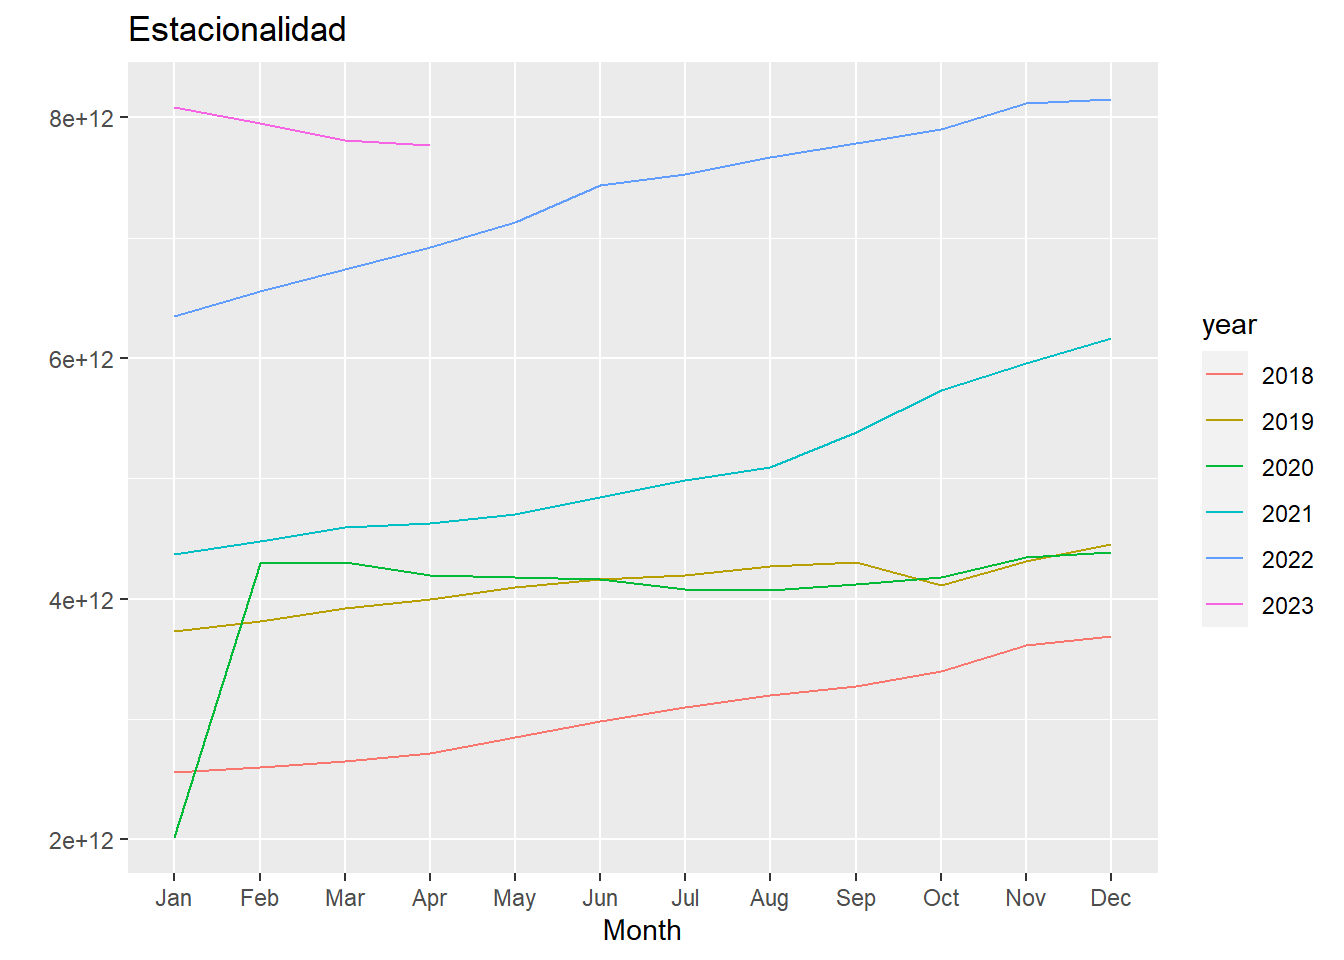
\includegraphics{bookdown-demo_files/figure-latex/unnamed-chunk-8-1.pdf}

\hypertarget{ahora-hagamos-una-decomposicion-del-objeto-y-la-graficamos-para-su-analisis}{%
\section{Ahora, hagamos una decomposicion del objeto y la graficamos para su analisis}\label{ahora-hagamos-una-decomposicion-del-objeto-y-la-graficamos-para-su-analisis}}

\begin{Shaded}
\begin{Highlighting}[]
\NormalTok{decomposicion }\OtherTok{\textless{}{-}} \FunctionTok{decompose}\NormalTok{(}\AttributeTok{x=}\NormalTok{indice.ts,}
                           \AttributeTok{type=} \StringTok{"additive"}\NormalTok{)}

\FunctionTok{plot}\NormalTok{(decomposicion)}
\end{Highlighting}
\end{Shaded}

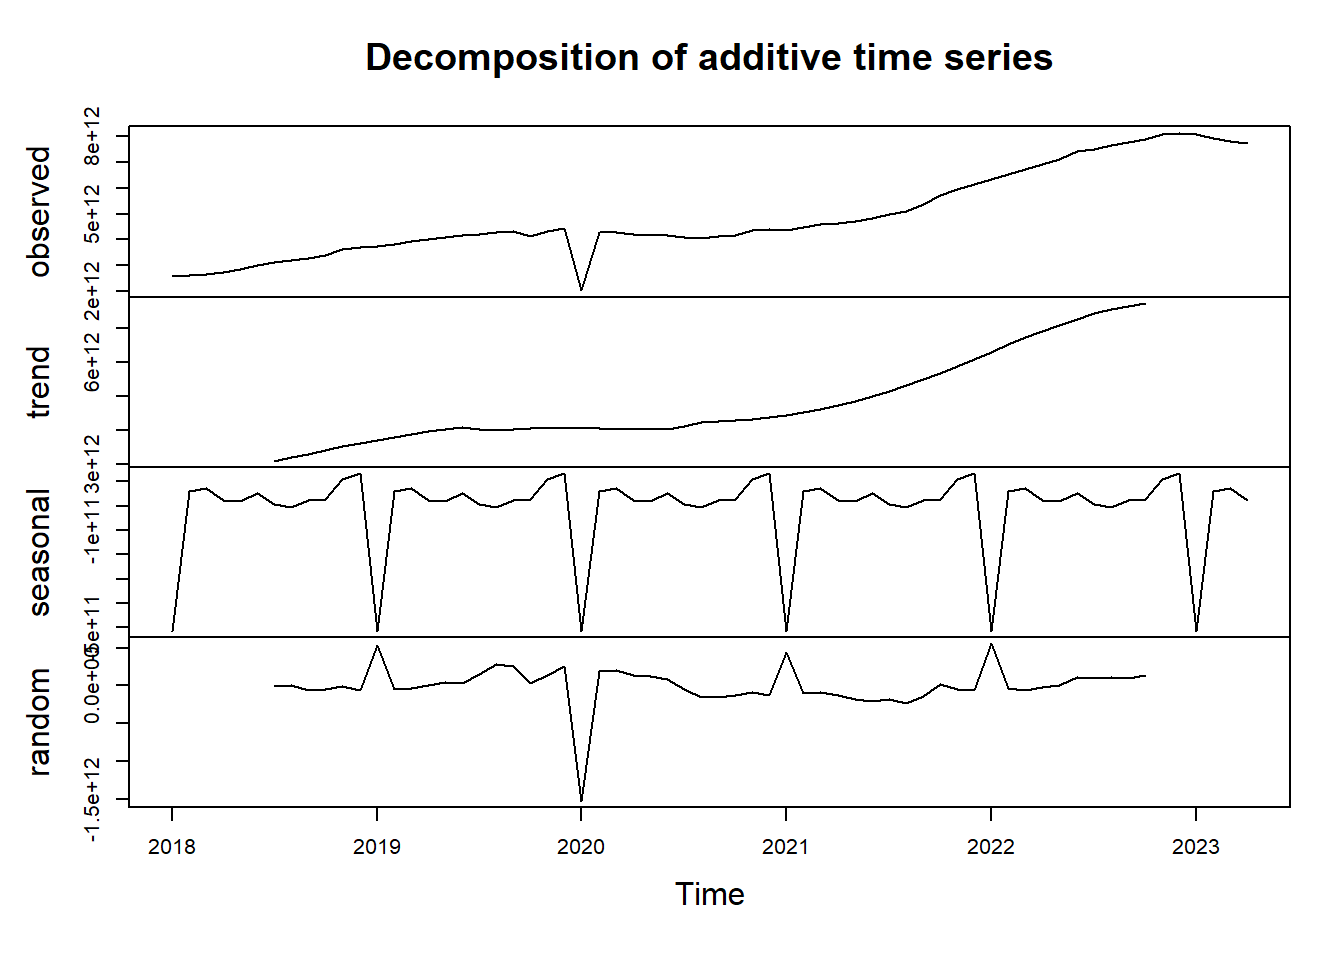
\includegraphics{bookdown-demo_files/figure-latex/unnamed-chunk-9-1.pdf}
David

\begin{Shaded}
\begin{Highlighting}[]
\DocumentationTok{\#\#\#\#\#\#\#\#\#\#\#\#\#\#\#\#\#\#\#\#\# descomposicion}


\CommentTok{\# Descomponer la serie de tiempo en sus componentes}
\NormalTok{descomposicion }\OtherTok{\textless{}{-}} \FunctionTok{decompose}\NormalTok{(indice.ts)}

\CommentTok{\# Obtener la componente de estacionalidad}
\NormalTok{estacionalidad }\OtherTok{\textless{}{-}}\NormalTok{ descomposicion}\SpecialCharTok{$}\NormalTok{seasonal}


\CommentTok{\# Convertir la componente de estacionalidad a un data frame}
\NormalTok{df\_estacionalidad }\OtherTok{\textless{}{-}} \FunctionTok{data.frame}\NormalTok{(}\AttributeTok{periodo =} \FunctionTok{time}\NormalTok{(estacionalidad), }\AttributeTok{valor =}\NormalTok{ estacionalidad)}

\CommentTok{\# Graficar la componente de estacionalidad}
\FunctionTok{ggplot}\NormalTok{(df\_estacionalidad, }\FunctionTok{aes}\NormalTok{(}\AttributeTok{x =}\NormalTok{ periodo, }\AttributeTok{y =}\NormalTok{ valor)) }\SpecialCharTok{+}
  \FunctionTok{geom\_line}\NormalTok{(}\AttributeTok{color =} \StringTok{"deepskyblue"}\NormalTok{, }\AttributeTok{size =} \DecValTok{1}\NormalTok{) }\SpecialCharTok{+}
  \FunctionTok{xlab}\NormalTok{(}\StringTok{"Periodo"}\NormalTok{) }\SpecialCharTok{+} \FunctionTok{ylab}\NormalTok{(}\StringTok{"Estacionalidad"}\NormalTok{) }\SpecialCharTok{+}
  \FunctionTok{ggtitle}\NormalTok{(}\StringTok{"Componente de estacionalidad de la serie de tiempo"}\NormalTok{)}
\end{Highlighting}
\end{Shaded}

\begin{verbatim}
## Warning: Using `size` aesthetic for lines was deprecated in ggplot2 3.4.0.
## i Please use `linewidth` instead.
## This warning is displayed once every 8 hours.
## Call `lifecycle::last_lifecycle_warnings()` to see where this warning was
## generated.
\end{verbatim}

\begin{verbatim}
## Don't know how to automatically pick scale for object of type <ts>. Defaulting
## to continuous.
## Don't know how to automatically pick scale for object of type <ts>. Defaulting
## to continuous.
\end{verbatim}

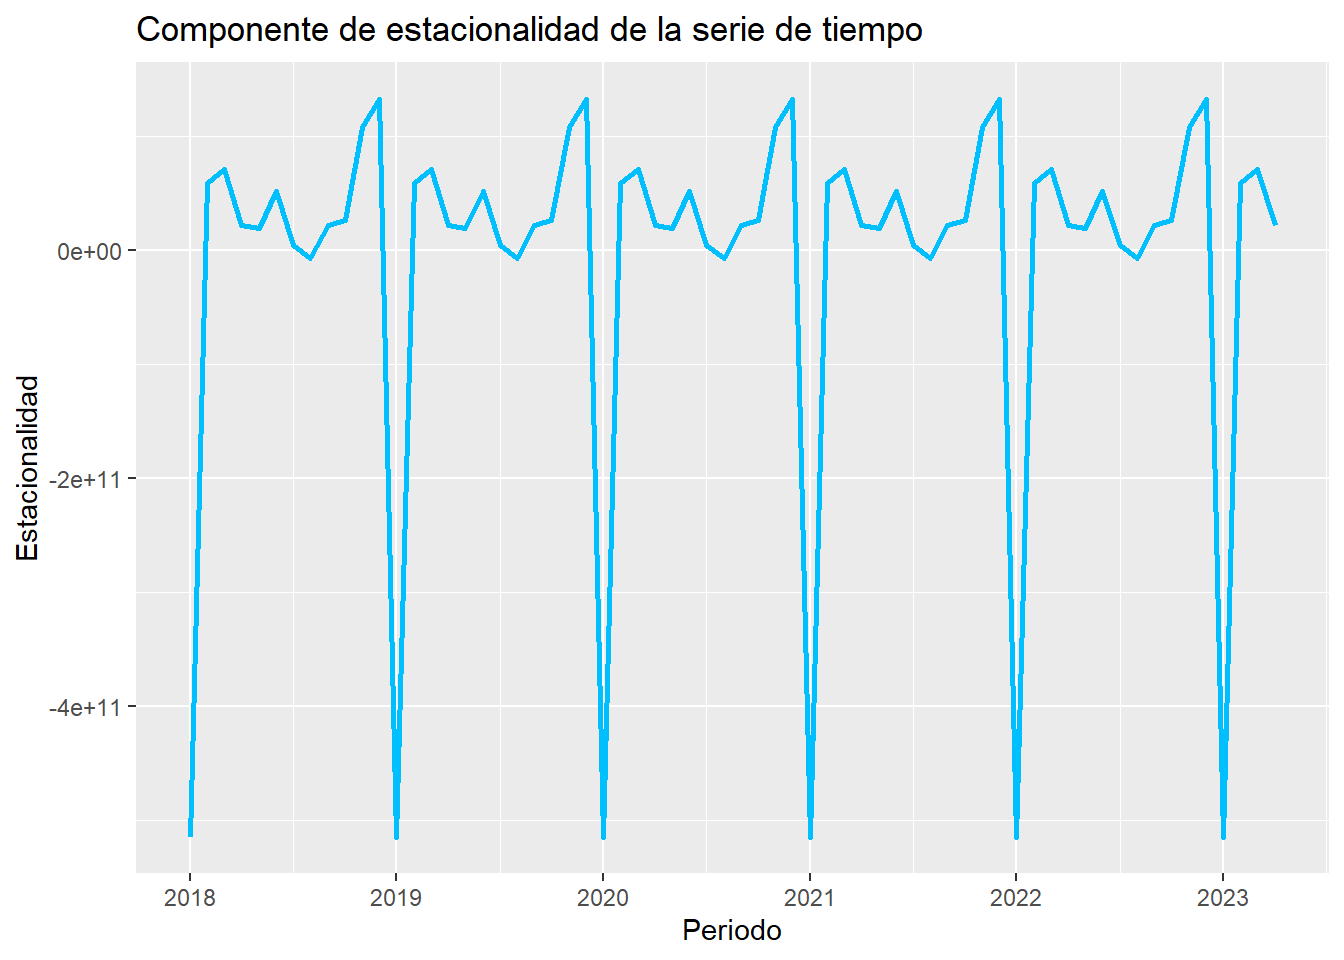
\includegraphics{bookdown-demo_files/figure-latex/unnamed-chunk-10-1.pdf}

\begin{Shaded}
\begin{Highlighting}[]
\DocumentationTok{\#\#\#\#\#\#\#\#\#\#\#\#\#\#\#\#\#\#\#\#\# diferenciación}

\CommentTok{\# Calcular la diferenciación}
\NormalTok{diferenciacion }\OtherTok{\textless{}{-}} \FunctionTok{diff}\NormalTok{(indice.ts)}


\CommentTok{\# Convertir la serie de tiempo diferenciada a un data frame}
\NormalTok{df\_diferenciacion }\OtherTok{\textless{}{-}} \FunctionTok{data.frame}\NormalTok{(}\AttributeTok{periodo =} \FunctionTok{time}\NormalTok{(diferenciacion), }\AttributeTok{valor =}\NormalTok{ diferenciacion)}

\CommentTok{\# Graficar la serie de tiempo diferenciada utilizando "ggplot2"}
\FunctionTok{ggplot}\NormalTok{(df\_diferenciacion, }\FunctionTok{aes}\NormalTok{(}\AttributeTok{x =}\NormalTok{ periodo, }\AttributeTok{y =}\NormalTok{ valor)) }\SpecialCharTok{+}
  \FunctionTok{geom\_line}\NormalTok{(}\AttributeTok{color =} \StringTok{"deepskyblue"}\NormalTok{, }\AttributeTok{size =} \DecValTok{1}\NormalTok{) }\SpecialCharTok{+}
  \FunctionTok{xlab}\NormalTok{(}\StringTok{"Periodo"}\NormalTok{) }\SpecialCharTok{+} \FunctionTok{ylab}\NormalTok{(}\StringTok{"Diferenciación"}\NormalTok{) }\SpecialCharTok{+}
  \FunctionTok{ggtitle}\NormalTok{(}\StringTok{"Serie de tiempo diferenciada"}\NormalTok{)}
\end{Highlighting}
\end{Shaded}

\begin{verbatim}
## Don't know how to automatically pick scale for object of type <ts>. Defaulting
## to continuous.
## Don't know how to automatically pick scale for object of type <ts>. Defaulting
## to continuous.
\end{verbatim}

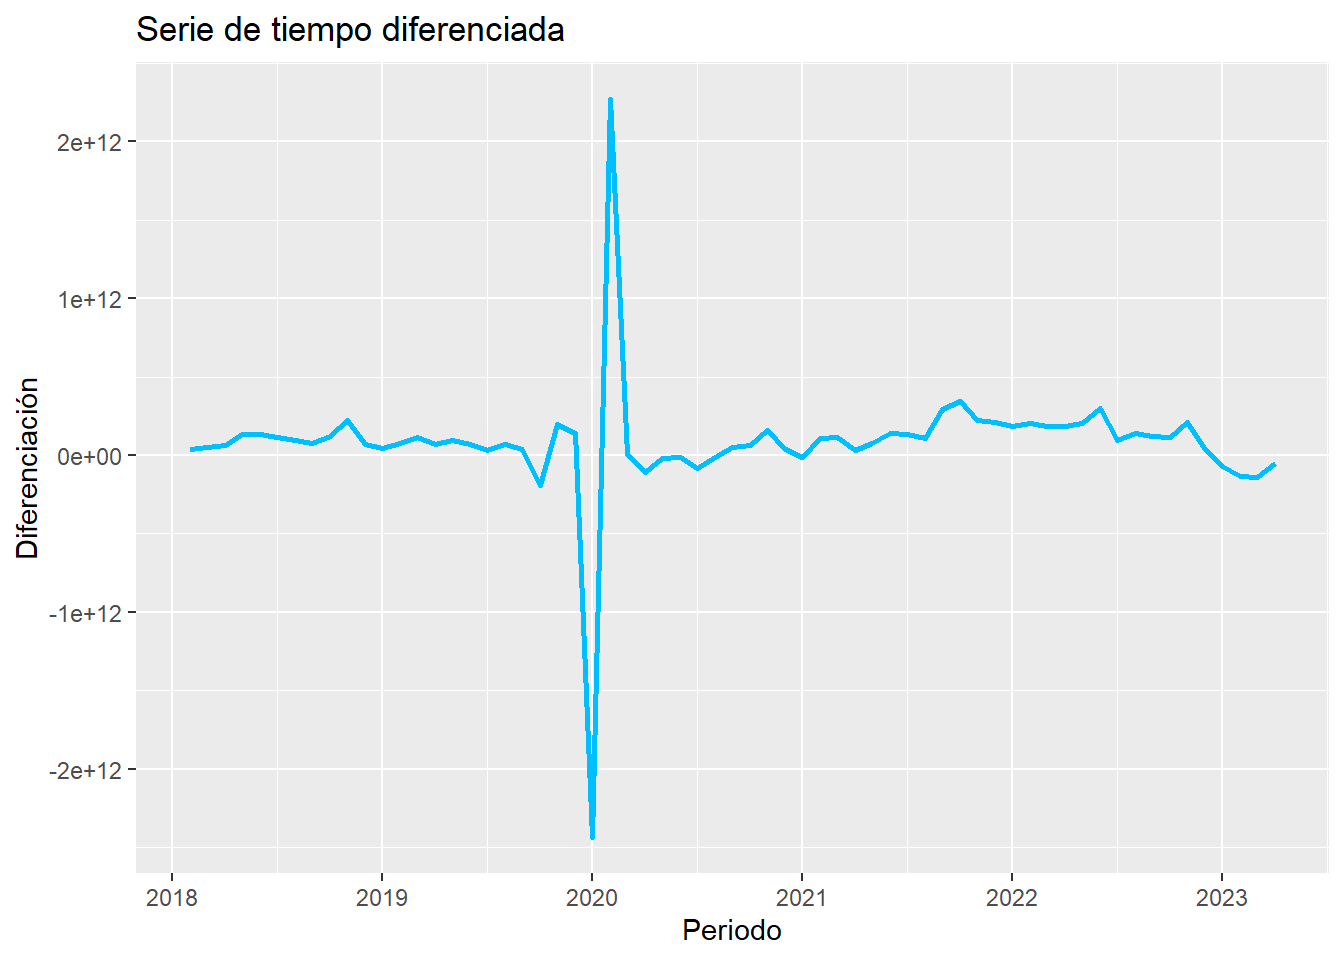
\includegraphics{bookdown-demo_files/figure-latex/unnamed-chunk-10-2.pdf}

\hypertarget{methods}{%
\chapter{Methods}\label{methods}}

We describe our methods in this chapter.

Math can be added in body using usual syntax like this

\hypertarget{math-example}{%
\section{math example}\label{math-example}}

\(p\) is unknown but expected to be around 1/3. Standard error will be approximated

\[
SE = \sqrt(\frac{p(1-p)}{n}) \approx \sqrt{\frac{1/3 (1 - 1/3)} {300}} = 0.027
\]

You can also use math in footnotes like this\footnote{where we mention \(p = \frac{a}{b}\)}.

We will approximate standard error to 0.027\footnote{\(p\) is unknown but expected to be around 1/3. Standard error will be approximated

  \[
  SE = \sqrt(\frac{p(1-p)}{n}) \approx \sqrt{\frac{1/3 (1 - 1/3)} {300}} = 0.027
  \]}

\hypertarget{applications}{%
\chapter{Applications}\label{applications}}

Some \emph{significant} applications are demonstrated in this chapter.

\hypertarget{example-one}{%
\section{Example one}\label{example-one}}

\hypertarget{example-two}{%
\section{Example two}\label{example-two}}

\hypertarget{final-words}{%
\chapter{Final Words}\label{final-words}}

We have finished a nice book.

  \bibliography{book.bib,packages.bib}

\end{document}
